\chapter{Bikini Ladies}
\label{ch:bikiniladies}
\index{dessert}
\index{cookies}
\index{molasses}
\index{Christmas}

\marginnote{
    \textbf{Makes 24 cookies} \\
    Prep time: 2+ hours \\
    Cook time: 7-10 minutes \\
    \vspace*{\baselineskip}

    \textbf{Ingredients for cookies} \\
    227g butter, room temperature \\
    1 cup brown sugar \\
    1/4 cup molasses \\
    1 egg \\
    2 3/4 cups all-purpose flour \\
    2 tsp cinnamon \\
    1/2 tsp cloves \\
    1 tbsp ginger \\
    2 tsp baking powder \\
    Pinch salt \\
    \vspace*{\baselineskip}
    
    \textbf{Ingredients for royal icing} \\
    2 egg whites \\
    2 tsp lemon juice \\
    3 cups icing sugar, sifted 
}
\begin{marginfigure}[20pt]
  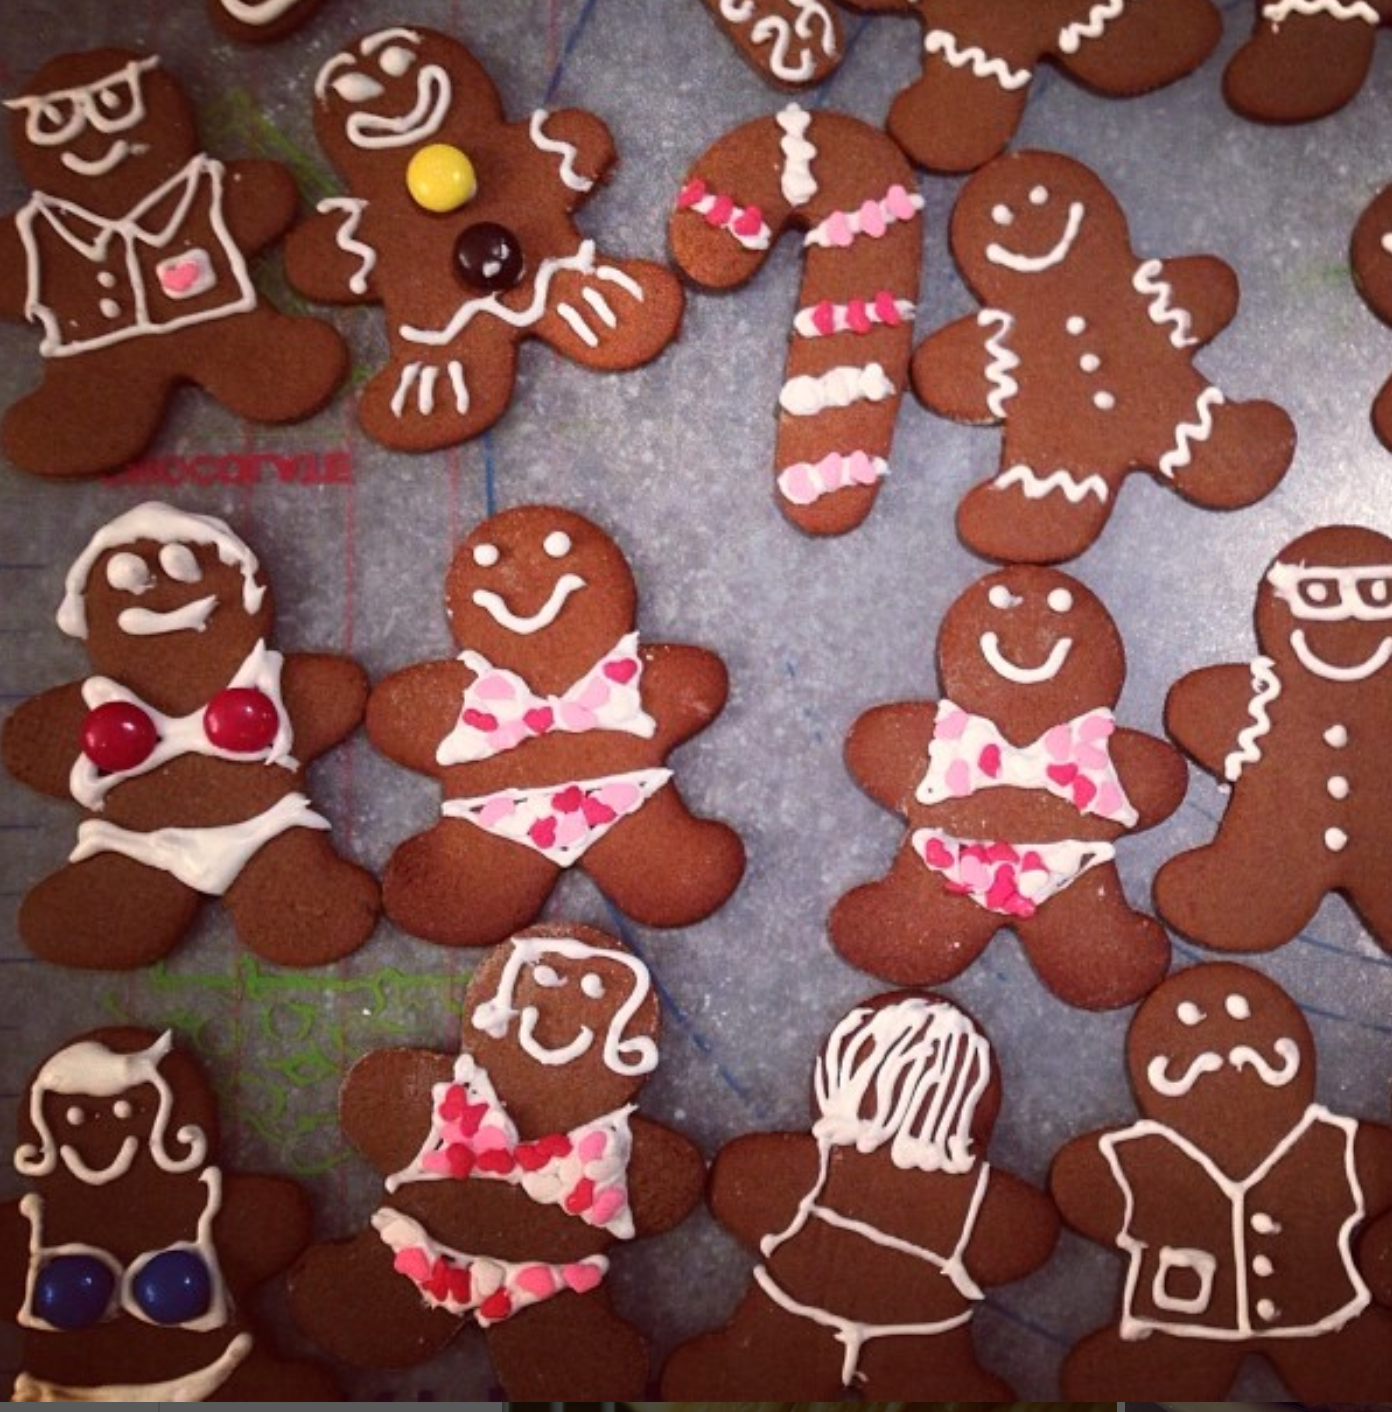
\includegraphics[width=60mm]{monanteras/images/Bikini ladies.png}
  \caption{Bikini Ladies and Hipsters}
\end{marginfigure}[20pt]

\textit{Gingerbread Cookies}

Family member: Elsa \& Helen

\newthought{Bikini Ladies} were created because we were dreaming of the beach while we were making gingerbread cookies during winter in Montreal!

\begin{enumerate}
    \item Using a mixer, cream the butter, brown sugar and molasses until pale and fluffy. Add egg and beat until well mixed.
    \item In a large bowl, whisk the flour, spices, baking powder and salt. 
    \item Gradually add the dry ingredients to the wet, scraping down the sides of the bowl. 
    \item Shape the dough into 2 rectangles, wrap in Saran Wrap and refrigerate for 1-2 hours. Meanwhile, make royal icing following the instructions below.
    \item Once the dough is cold, flour the counter and roll it out. Keep the other dough in the refrigerator. Cut into desired shapes using Christmassy cookie cutters and place onto a baking sheet lined with parchment paper. 
    \item Chill for 30 minutes, then bake at 350\degree F for 10-12 minutes, turning midway.
    \item To make the royal icing, whisk the egg whites with lemon juice in a mixing bowl. Add the sifted icing sugar in 1 time and whisk until all is incorporated, stopping the mixer once to scrape down the sides of the bowl. If the icing is too runny, add a little more sifted icing sugar. 
    \item Cover the bowl with a damp towel to avoid a crust forming and drying out of the icing while you cook the cookies.
    \item Once the cookies have cooled down, decorate the Bikini Ladies using icing, sprinkles, candies and M \& Ms.
\end{enumerate}
